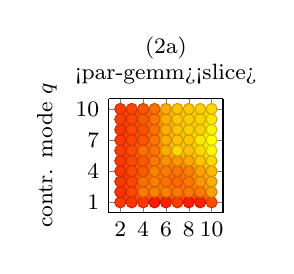
\begin{tikzpicture}
\begin{axis}
[
width=0.25\textwidth,
height=0.25\textwidth,
style={font=\footnotesize},
grid=major,
grid style={dotted},
align=center,
%xlabel={tensor order},
ylabel={contr. mode $q$},
title={(2a)\\\tss{<par-gemm><slice>}}, %  pargemm<slice>, asymmetric, row-major, mkl
title style={yshift=-1ex},
scaled ticks=false,
zlabel={GFlops/core},
view={0}{90}, 
%view={-45}{45}, 
ytick={1,4,7,10},
xtick={2,4,6,8,10},
xmin=1, xmax=11,
ymin=0, ymax=11,
try min ticks=8,
zmin=0, zmax=55,
point meta min=0, point meta max=55,
colormap/hot, 
samples=55,
]
\addplot3[contour filled={number=100},scatter,shader=flat,samples=55]
coordinates{
(2.000,1.000,46.317) (2.000,2.000,47.467) (2.000,3.000,46.785) (2.000,4.000,46.908) (2.000,5.000,46.657) (2.000,6.000,45.822) (2.000,7.000,46.501) (2.000,8.000,47.166) (2.000,9.000,45.817) (2.000,10.000,45.838) 

(3.000,1.000,46.799) (3.000,2.000,44.592) (3.000,3.000,44.972) (3.000,4.000,44.132) (3.000,5.000,44.473) (3.000,6.000,43.555) (3.000,7.000,45.048) (3.000,8.000,44.306) (3.000,9.000,44.715) (3.000,10.000,44.711) 

(4.000,1.000,46.289) (4.000,2.000,37.746) (4.000,3.000,39.173) (4.000,4.000,42.161) (4.000,5.000,42.303) (4.000,6.000,39.003) (4.000,7.000,42.644) (4.000,8.000,43.034) (4.000,9.000,41.854) (4.000,10.000,42.895) 

(5.000,1.000,50.964) (5.000,2.000,36.480) (5.000,3.000,37.083) (5.000,4.000,36.474) (5.000,5.000,37.539) (5.000,6.000,38.234) (5.000,7.000,38.204) (5.000,8.000,38.503) (5.000,9.000,37.973) (5.000,10.000,38.626) 

(6.000,1.000,49.775) (6.000,2.000,36.594) (6.000,3.000,38.549) (6.000,4.000,37.212) (6.000,5.000,34.515) (6.000,6.000,30.085) (6.000,7.000,30.745) (6.000,8.000,30.647) (6.000,9.000,30.171) (6.000,10.000,30.565) 

(7.000,1.000,46.098) (7.000,2.000,37.478) (7.000,3.000,39.858) (7.000,4.000,38.195) (7.000,5.000,33.103) (7.000,6.000,23.667) (7.000,7.000,26.990) (7.000,8.000,27.232) (7.000,9.000,26.693) (7.000,10.000,27.254) 

(8.000,1.000,50.490) (8.000,2.000,37.502) (8.000,3.000,37.745) (8.000,4.000,36.398) (8.000,5.000,31.315) (8.000,6.000,27.314) (8.000,7.000,26.440) (8.000,8.000,25.665) (8.000,9.000,25.704) (8.000,10.000,25.867) 

(9.000,1.000,49.745) (9.000,2.000,37.042) (9.000,3.000,33.158) (9.000,4.000,31.522) (9.000,5.000,26.570) (9.000,6.000,23.876) (9.000,7.000,21.588) (9.000,8.000,24.772) (9.000,9.000,24.220) (9.000,10.000,24.867) 

(10.000,1.000,43.680) (10.000,2.000,31.533) (10.000,3.000,30.229) (10.000,4.000,28.157) (10.000,5.000,23.743) (10.000,6.000,19.455) (10.000,7.000,18.637) (10.000,8.000,19.922) (10.000,9.000,21.995) (10.000,10.000,23.892) 


};
\end{axis}
\end{tikzpicture}
\hfill
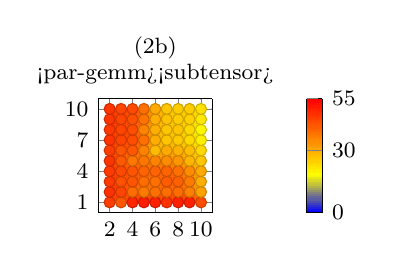
\begin{tikzpicture}
\begin{axis}
[
width=0.25\textwidth,
height=0.25\textwidth,
style={font=\footnotesize},
grid=major,
grid style={dotted},
align=center,
%xlabel={tensor order},
%ylabel={contr. mode (q)},
title={(2b)\\\tss{<par-gemm><subtensor>}}, %  pargemm<subtensor>, asymmetric, mkl, row.major
title style={yshift=-1ex},
scaled ticks=false,
zlabel={GFlops},
view={0}{90}, 
ytick={1,4,7,10},
xtick={2,4,6,8,10},
xmin=1, xmax=11,
ymin=0, ymax=11,
try min ticks=8,
zmin=0, zmax=55,
point meta min=0, point meta max=55,
colormap/hot, 
samples=55,
colorbar sampled,
colorbar/width=0.2cm,
colorbar style={
point meta min=0, point meta max=55,
samples=55,
font=\footnotesize,
ytick={0,30,55},
yticklabels={0,30,55},
%title={\scriptsize Gflops},
%ylabel={\scriptsize Gflops},
}
]
\addplot3[contour filled={number=100},scatter,shader=flat,samples=55]
coordinates{

(2.000,1.000,46.024) (2.000,2.000,47.499) (2.000,3.000,46.518) (2.000,4.000,46.647) (2.000,5.000,46.939) (2.000,6.000,45.807) (2.000,7.000,46.788) (2.000,8.000,46.201) (2.000,9.000,46.824) (2.000,10.000,46.817) 

(3.000,1.000,41.968) (3.000,2.000,44.618) (3.000,3.000,43.239) (3.000,4.000,44.176) (3.000,5.000,42.190) (3.000,6.000,42.685) (3.000,7.000,44.634) (3.000,8.000,44.551) (3.000,9.000,45.078) (3.000,10.000,44.656) 

(4.000,1.000,49.206) (4.000,2.000,39.114) (4.000,3.000,42.621) (4.000,4.000,42.869) (4.000,5.000,37.872) (4.000,6.000,41.893) (4.000,7.000,43.549) (4.000,8.000,43.776) (4.000,9.000,43.074) (4.000,10.000,44.055) 

(5.000,1.000,50.432) (5.000,2.000,37.339) (5.000,3.000,39.583) (5.000,4.000,40.371) (5.000,5.000,37.481) (5.000,6.000,36.183) (5.000,7.000,38.874) (5.000,8.000,36.295) (5.000,9.000,38.334) (5.000,10.000,38.828) 

(6.000,1.000,49.563) (6.000,2.000,39.033) (6.000,3.000,38.729) (6.000,4.000,40.488) (6.000,5.000,35.766) (6.000,6.000,28.574) (6.000,7.000,30.137) (6.000,8.000,29.909) (6.000,9.000,30.071) (6.000,10.000,30.335) 

(7.000,1.000,47.837) (7.000,2.000,39.558) (7.000,3.000,41.754) (7.000,4.000,40.236) (7.000,5.000,34.661) (7.000,6.000,30.281) (7.000,7.000,26.674) (7.000,8.000,26.594) (7.000,9.000,27.319) (7.000,10.000,26.694) 

(8.000,1.000,49.852) (8.000,2.000,39.408) (8.000,3.000,41.192) (8.000,4.000,38.730) (8.000,5.000,33.342) (8.000,6.000,29.655) (8.000,7.000,26.196) (8.000,8.000,26.772) (8.000,9.000,25.778) (8.000,10.000,25.490) 

(9.000,1.000,49.752) (9.000,2.000,36.678) (9.000,3.000,36.985) (9.000,4.000,34.654) (9.000,5.000,29.039) (9.000,6.000,27.701) (9.000,7.000,24.123) (9.000,8.000,24.053) (9.000,9.000,25.007) (9.000,10.000,25.359) 

(10.000,1.000,43.556) (10.000,2.000,31.723) (10.000,3.000,30.114) (10.000,4.000,30.474) (10.000,5.000,26.695) (10.000,6.000,24.184) (10.000,7.000,20.683) (10.000,8.000,19.787) (10.000,9.000,21.875) (10.000,10.000,22.884) 


};
\end{axis}
\end{tikzpicture}
\hfill
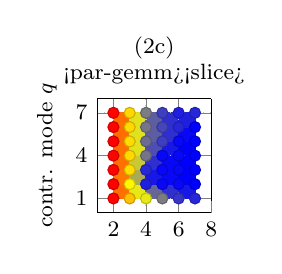
\begin{tikzpicture}
\begin{axis}
[
width=0.25\textwidth,
height=0.25\textwidth,
style={font=\footnotesize},
grid=major,
grid style={dotted},
align=center,
%xlabel={tensor order},
ylabel={contr. mode $q$},
title={(2c)\\\tss{<par-gemm><slice>}}, %  pargemm<slice>, symmetric, row-major
title style={yshift=-1ex},
scaled ticks=false,
zlabel={GFlops},
view={0}{90}, 
ytick={1,4,7,10},
xtick={2,4,6,8},
xmin=1, xmax=8,
ymin=0, ymax=8,
try min ticks=8,
zmin=0, zmax=55,
point meta min=0, point meta max=55,
colormap/hot, 
samples=55
]
\addplot3[contour filled={number=100},scatter,shader=flat,samples=55]
coordinates{

(2.000,1.000,54.069) (2.000,2.000,54.524) (2.000,3.000,54.079) (2.000,4.000,54.441) (2.000,5.000,54.500) (2.000,6.000,54.168) (2.000,7.000,54.447) 

(3.000,1.000,27.294) (3.000,2.000,19.589) (3.000,3.000,23.485) (3.000,4.000,23.978) (3.000,5.000,23.522) (3.000,6.000,24.035) (3.000,7.000,23.660) 

(4.000,1.000,16.871) (4.000,2.000,2.541) (4.000,3.000,2.842) (4.000,4.000,8.714) (4.000,5.000,8.244) (4.000,6.000,8.648) (4.000,7.000,8.818) 

(5.000,1.000,8.873) (5.000,2.000,0.844) (5.000,3.000,0.856) (5.000,4.000,0.854) (5.000,5.000,4.875) (5.000,6.000,5.034) (5.000,7.000,4.445) 

(6.000,1.000,4.355) (6.000,2.000,0.570) (6.000,3.000,0.575) (6.000,4.000,0.623) (6.000,5.000,0.593) (6.000,6.000,2.899) (6.000,7.000,2.728) 

(7.000,1.000,3.255) (7.000,2.000,0.244) (7.000,3.000,0.159) (7.000,4.000,0.251) (7.000,5.000,0.264) (7.000,6.000,0.258) (7.000,7.000,3.065) 


};
\end{axis}
\end{tikzpicture}
\hfill
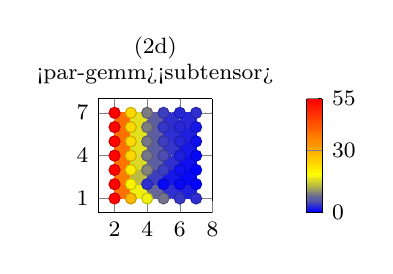
\begin{tikzpicture}
\begin{axis}
[
width=0.25\textwidth,
height=0.25\textwidth,
style={font=\footnotesize},
grid=major,
grid style={dotted},
align=center,
%xlabel={tensor order},
%ylabel={contr. mode (q)},
title={(2d)\\\tss{<par-gemm><subtensor>}}, %  pargemm<subtensor>, symmetric, row-major
title style={yshift=-1ex},
scaled ticks=false,
zlabel={GFlops},
view={0}{90}, 
%view={-45}{45}, 
ytick={1,4,7,10},
xtick={2,4,6,8},
xmin=1, xmax=8,
ymin=0, ymax=8,
try min ticks=8,
zmin=0, zmax=55,
point meta min=0, point meta max=55,
colormap/hot, 
colorbar sampled,
colorbar/width=0.2cm,
colorbar style={
point meta min=0, point meta max=55,
font=\footnotesize,
ytick={0,30,55},
yticklabels={0,30,55},
samples=55
%title={\scriptsize Gflops},
%ylabel={\scriptsize Gflops},
}
]
\addplot3[contour filled={number=100},scatter,shader=flat,samples=55]
coordinates{

(2.000,1.000,54.044) (2.000,2.000,54.235) (2.000,3.000,53.780) (2.000,4.000,54.392) (2.000,5.000,54.142) (2.000,6.000,53.918) (2.000,7.000,54.583) 

(3.000,1.000,28.060) (3.000,2.000,19.851) (3.000,3.000,21.251) (3.000,4.000,23.673) (3.000,5.000,23.690) (3.000,6.000,23.943) (3.000,7.000,23.887) 

(4.000,1.000,17.114) (4.000,2.000,3.369) (4.000,3.000,9.529) (4.000,4.000,8.731) (4.000,5.000,8.373) (4.000,6.000,8.989) (4.000,7.000,8.866) 

(5.000,1.000,8.728) (5.000,2.000,0.898) (5.000,3.000,4.591) (5.000,4.000,5.693) (5.000,5.000,4.813) (5.000,6.000,4.240) (5.000,7.000,4.917) 

(6.000,1.000,4.370) (6.000,2.000,0.573) (6.000,3.000,1.397) (6.000,4.000,2.626) (6.000,5.000,2.874) (6.000,6.000,2.815) (6.000,7.000,2.828) 

(7.000,1.000,3.777) (7.000,2.000,0.243) (7.000,3.000,0.303) (7.000,4.000,0.649) (7.000,5.000,1.255) (7.000,6.000,1.973) (7.000,7.000,3.407) 



};
\end{axis}
\end{tikzpicture}